\chapter{Electrical Power System}
\label{chap:eps}

\section{Introduction}
\label{sec:introduction}

The \ac{EPS} will provide sufficient power to the motors, communication system and payloads. Power is generated from solar cells and stored in batteries. DC-DC regulators are used to control the operating voltage of the solar cell and to provide regulated voltages to payloads and onboard computers.
%
\subsection{Changes from PDR to CDR}
\label{sec:changes_pdr_to_cdr}
%
The U-SPACE \ac{PDR} for the \ac{EPS} is documented in \cite{PDR}. Table \ref{tab:pdr_to_cdr} lists the major \ac{EPS} design changes between the \ac{PDR} and the \ac{CDR} and the argumentations behind these design changes.

\begin{table}[H]
\centering
\caption{U-SPACE \ac{EPS} design changes from PDR to CDR}
\label{tab:pdr_to_cdr}
\begin{tabular}{p{0.25\textwidth}p{0.25\textwidth}p{0.5\textwidth}}
\hline
\textbf{Area of change }& \textbf{Changed parameter }& \textbf{Argumentation for change}\\
\hline
Total power budget & increased to $>40\,W$ & Increased airship total mass and size\\
Solar cells & New part & Old solar cell was much heavier than listed in manufacturer datasheet due to a glass cover\\
Total system cost & increased to $>12000\,SEK$ & Increased power requirements and new light-weight solar cells are more expensive\\
Solar cell mounting & New part & New solar cell is flexible instead of rigid and can be mounted with \ac{PSA}\\
\hline
\end{tabular}
\end{table} 

\section{Functional and Technical Requirements}

\subsection{Functional Requirements}
%What function(s) does the subsystem have to fulfill?
%
Below are listed the primary functional requirements for the \ac{EPS}:
%
\begin{itemize}
\item Provide adequate power to motors and payload
\item Proof that flying on solar energy is possible i.e more power produced than consumed
\end{itemize}
%
Additional desired requirements are:
%
\begin{itemize}
\item Scalability to higher power levels
\item Flexible and robust design, allowing flight in more extreme conditions (altitude, weather etc.)
\item Provide adequate protection circuits for battery and loads
\item Optimal design and high performance to increase power capability and minimize system mass
\end{itemize}
%
%
\subsection{Technical Requirements}
%What technical requirements constrain the subsystem design? - e.g. mass, power, strength, stability etc.
%
The \ac{EPS} technical requirements are listed in table \ref{tab:technical_requirements}.
%
\begin{table}[H]
\centering
\caption{Technical requirements for the \ac{EPS}}
\label{tab:technical_requirements}
\begin{minipage}{\textwidth}
\begin{tabular}{p{0.4\textwidth}p{0.4\textwidth}}
\hline
Minimum power output & $40\,W$\\
Maximum mass & $1000\,g$(including solar arrays)\\
Maximum cost & $5000\,SEK$\footnote{Initial budget for 2 students.}\\
%Maximum internal power dissipation & $<500\,mW$\\
Output voltages & $6.0-9.2\,V$(un-regulated), $5\,V$( regulated)\\
Maximum output current (worst case) & $10.5\,A$\\
Regulator phase margin & $60\,deg$\\
Regulator gain margin & $10\,dB$\\
Control loop bandwidth & $>10\,kHz$\\
Operational temperature & $-20^{\circ}C\,to +25^{\circ}C$\\
Battery capacity & $>5\,Wh$\\
\hline
\end{tabular}\par
\vspace{-0.75\skip\footins}
\renewcommand{\footnoterule}{}
\end{minipage}
\end{table}
%
%\subsection{Mission and Environmental Constraints}
%\label{subsec:environmental_requirements}
%This section discusses some of the challenges opposed by the mission and the parameters of operation environment and how these will influence the \ac{EPS} design constraints.
%
%\subsubsection*{Solar Array Temperature}
%Temperature variation of the solar panels, significantly changes the solar panels characteristics and of main importance the location of the \ac{MPP}. In \cite{PDR} using the temperature coefficient of the open-circuit voltage of a proposed solar cell, the decrease in power output from the cell when the temperature goes from $-20^{\circ}C$ to $+25^{\circ}C$ was estimated to around $15-20\%$. The temperature characteristics of the chosen solar cells [reference] are not provided by the manufacturer, hence these should be tested in order to estimate the solar cell sensitivity to temperature changes. To mitigate this issue, a \ac{MPPT} is applied which will be explained in section [reference].
%
%
\subsection{Expected Performance}
%What are the expected performances of the subsystem, as related to the requirements above? (maybe including some margins)
%
\begin{table}[H]
\centering
\caption{Expected performance of the \ac{EPS}}
\label{tab:expected_performance}
\begin{minipage}{\textwidth}
\begin{tabular}{p{0.55\textwidth}p{0.35\textwidth}}
\hline
Power conversion efficiency(overall) & $80-90\%$\\
Power output(overall) & $\sim 57-65\,W$\\
Battery capacity & $7.3\,Wh$\\
Mass & $\sim910\,g$\\
Total cost & $\sim12000\,SEK$\footnote{Solar cells are significantly more expensive than anticipated. A request for more funds is under preparation.}\\
\hline
\end{tabular}\par
\vspace{-0.75\skip\footins}
\renewcommand{\footnoterule}{}
\end{minipage}
\end{table}

\section{Critical Design}
\label{sec:critical_design}

This section describes in more detail the \ac{EPS} design. A simple block diagram of the \ac{EPS} design is shown in Figure \ref{fig:EPS_diagram_simple}.

\begin{figure}[H]
\centering
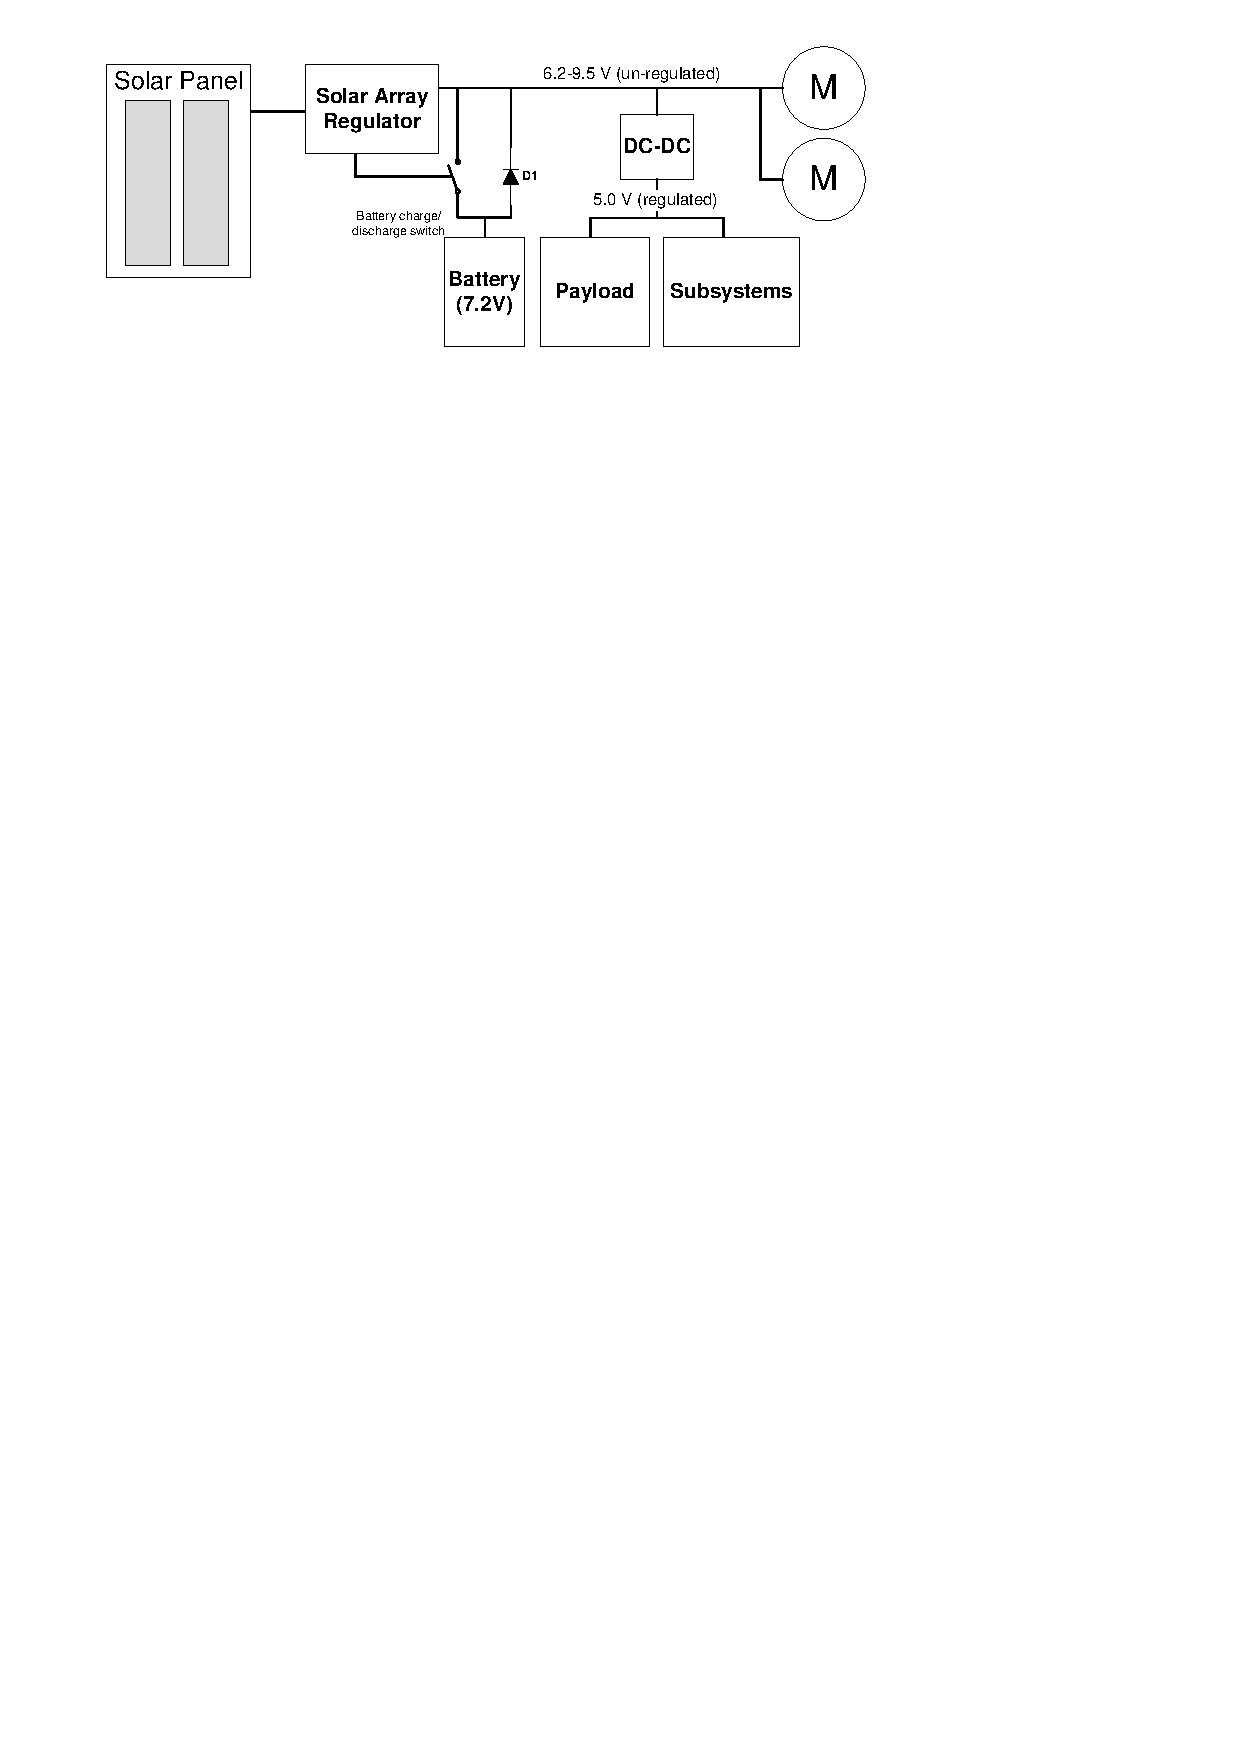
\includegraphics[width=\textwidth]{figures/fig_PDR_EPSdiagram}
\caption{\ac{EPS} simple blockdiagram}
\label{fig:EPS_diagram_simple}
\end{figure}
%
%
\subsection{Solar Array Design}
%Bypass diodes on SA to mitegate shadowing problems
%Cross-strapping of solar cells?
%\subsubsection*{Solar Array Shading}
%Bypass diodes can be used to partly mitigate this issue as well as using \ac{MPPT}. Otherwise it could be necessary to ensure that the airship structure cannot cast shadows on the panels and that the airship only fly above or away from landscape objects.
As was mentioned in section \ref{sec:changes_pdr_to_cdr}, a new solar cell has been selected. This solar cell is shown in Figure \ref{fig:solar_cell} and Table \ref{tab:solar_cell_spec} lists the important specifications for this cell.
%
\begin{figure}[H]
\centering
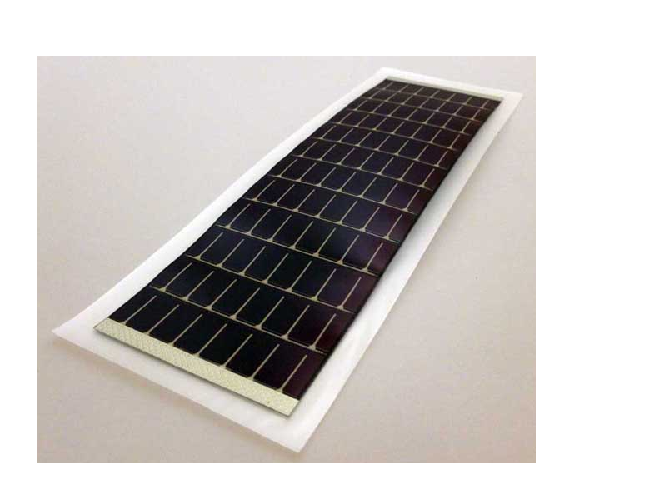
\includegraphics[width=0.3\textwidth]{figures/SolarCell_RC7-2_Powerfilm}
\caption{Chosen solar cell}
\label{fig:solar_cell}
\end{figure}
%
\begin{table}[H]
\centering
\caption{Specifications of chosen solar cell}
\label{tab:solar_cell_spec}
\begin{minipage}{\textwidth}
\begin{tabular}{ll}
\hline
Nominal output current & $100\,mA$\\
Nominal output voltage & $7.2V$\\
Nominal output power & $0.72\,W$\\
Dimensions & $270\,mm\:\times\:90\,mm\:\times\:0.2\,mm$\\
Weight & $7.6\,g$\\
No. of required cells $100$\footnote{\cite{avnetexpress} offers good discount for +100 units order}\\
Total solar panel area & $2.43\,m^2$ (assuming $100\,\%$ fill factor)\\
\hline
\end{tabular}\par
\vspace{-0.75\skip\footins}
\renewcommand{\footnoterule}{}
\end{minipage}
\end{table}
%
%
The solar panels will be configured with two series-connected solar cells thus having an output voltage of: 
%
\begin{equation}
V_{panel,out}=14.4\,V
\end{equation}
%
%
\subsection{Battery Design}
%
Two Panasonic PA-L60.K02 \cite{panasonic} Li-ion batteries are used. The battery has the following important specifications:
%
\begin{table}[H]
\centering
\caption{Specification of chosen battery}
\label{tab:proposed_battery}
\begin{tabular}{ll}
\hline
Chemistry & Li-ion\\
Nominal voltage & $3.6\,V$\\
Capacity & $1.03\,Ah$ / $3.61\,Wh$\\
Weight & $25\,g$\\
Dimensions & $56\,mm\:\times\:34.2\,mm\:\times\:5.8\,mm$\\
Maximum charge current & $970\,mA$\\
Maximum discharge current (continuous) & $1.455\,A$\\
\hline
\end{tabular}
\end{table}
%
%
\subparagraph*{Future Recommendations}
%
The chosen type of Li-ion battery supports only a relative low charge- and discharge rate of about $1\,C$. For bigger battery capacity and higher loads, it is recommended to use a battery like \cite{rcflight_battery} which provides much higher discharge rates ($>20\,C$) and also cheaper price per Wh. Only disadvantage  is a mass increase of around $15-25\%$.
%
\subsubsection{Battery Charge Regulator}
%
From the battery datasheet, maximum charge current is $I_{REG}=970\,mA$. From the \ac{BCR} datasheet, the minimum current sense resistor value is calculated as
%
\begin{equation}
\begin{split}
R_{sense}=&\dfrac{V_{FCS}}{I_{REG}}\\
R_{sense}=&\dfrac{120\,mV}{970\,mA}=123\,m\Omega
\end{split}
\end{equation}
%
The required thermal rating of the pass transistor is calculated as
%
\begin{equation}
P_{max}=(V_{in,max}-V_{bat,min})\cdot I_{charge}=(9.5\,V-5.5\,V)\cdot 970\,mA=3.88\,W
\end{equation}
%
\subsubsection{Battery Temperature Monitoring}
%
The \ac{BCR} chip includes a temperature monitoring feature. The battery is rated, in charge-mode, to temperature in the interval $10-45^{\circ}C$. The maximum allowed temperature is set slightly lower to $40^{\circ}C$. The Li-ion battery has a build-in \ac{NTC} thermistor with $B=3980\,K$ and $R_{25}=10k\,\Omega$. The required restance values of the temperature control resistors are determined from the \ac{BCR} chip datasheet as 
%
\begin{equation}
\begin{split}
R_{cold}&=R_{25}e^{B(\dfrac{1}{T}-\dfrac{1}{T_0}}=10\,k\Omega e^{3980\,K(\dfrac{1}{283	\,K}-\dfrac{1}{298\,K})}=20.3\,k\Omega\\
R_{hot}&=10\,k\Omega e^{3980\,K(\dfrac{1}{313	\,K}-\dfrac{1}{298\,K})}=5.3\,k\Omega\\
R_{T1}&=2\dfrac{R_{cold}R_{hot}}{R_{cold}-R_{hot}}=14.2\,k\Omega\\
R_{T2}&=2\dfrac{R_{cold}R_{hot}}{R_{cold}-3R_{hot}}=47.8\,k\Omega
\end{split}
\end{equation}

%
\subsubsection{Battery Discharge Current Limiter}
%
The selected MOSFET has a typical gate threshold voltage of $V_{Gth}=550\,mV$. The chosen \ac{BJT} has a typical collector-emitter voltage drop of $V_{CE}=120\,mV$. The battery is rated for a maximum discharge current of $I_{discharge}=1.455\,A$. The required current sense resistor is then calculated as 
%
\begin{equation}
\begin{split}
V_{sense}&=V_{Gth}-V_{CE}=550\,mV-120\,mV=430\,mV \Rightarrow\\
R_{sense}&=\dfrac{V_{sense}}{I_{discharge}}=\dfrac{430\,mV}{1.455\,A}=295\,m\Omega
\end{split}
\end{equation}
%
The exact required resistance must be determined by testing the precise parameters of the discrete components.
%
%
%
\subsection{Maximum Power Point Tracking Regulator}
%Which design concepts are considered? - What are the advantages/disadvantages for each concept?
%Decide on MPPT algorithm (using analog circuits?)
%DC-DC regulator topology (Buck, Boost, Buck-Boost etc.)
%
In \cite{PDR} it was decided to use a \ac{MPPTU} for the \ac{APR} due to its high efficiency and robustness to changing environmental constraints.

In first step, only the DC-DC converter will be implemented. When time and resources allows the \ac{MPPT} part will be added.
A simple buck DC-DC converter topology is used, comprising a transistor, free-wheel diode, inductor and output capacitor. 
When the full \ac{MPPTU} is implemented, it will operate in three different operation regions:
%
\begin{itemize}
\item Battery discharge {MPPT} - when the solar array input power is insufficient to cover the load power demand, the battery is slowly discharged in order to maintain the output voltage.
\item Battery charge {MPPT} - when the solar array input is greater than the load power, the excessive power is used to recharge the battery.
\item Input power limitation - when the battery is fully charged, the regulator will operate the solar array at a non-optimal voltage, thus limiting the input power to keep the output voltage constant. The extra potential input power is dissipated as heat externally on the solar arrays.
\end{itemize}
%
\begin{figure}[H]
\centering
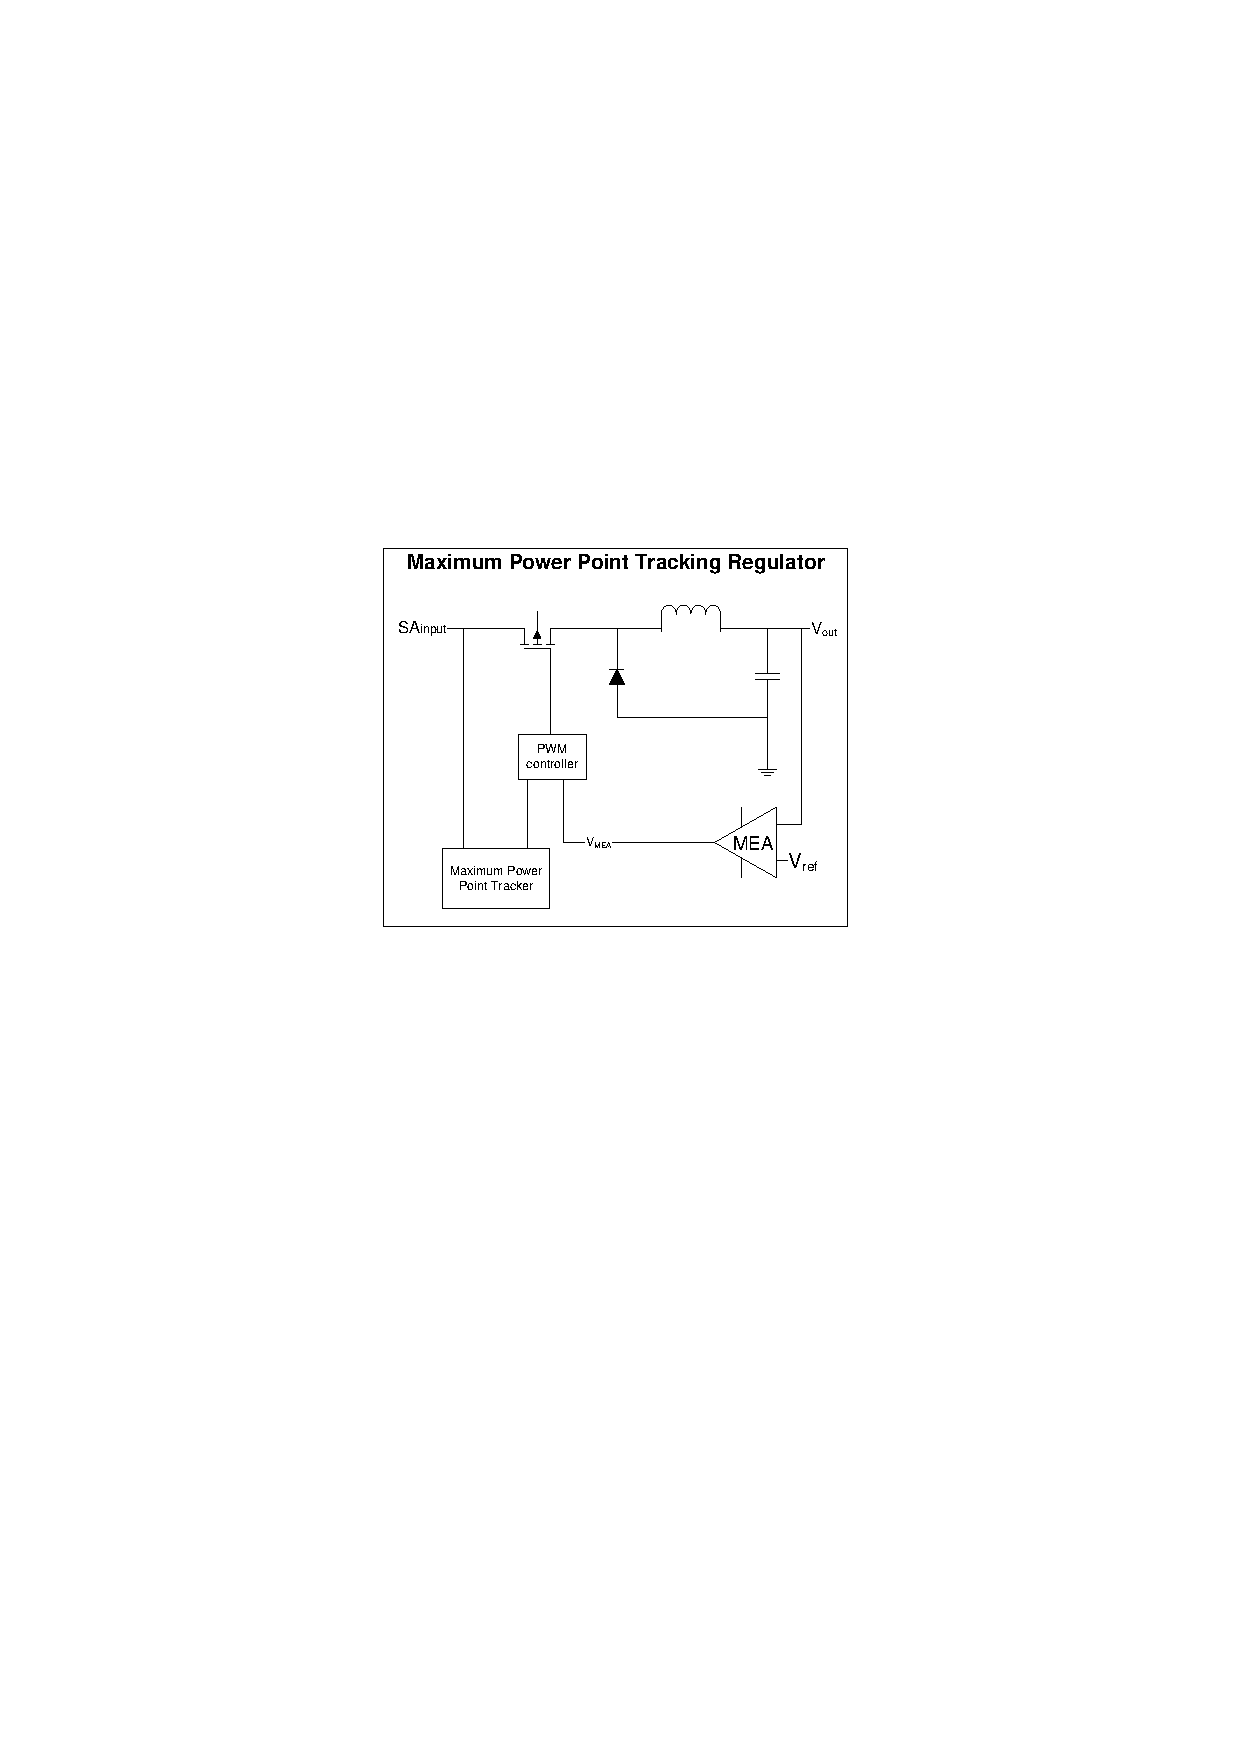
\includegraphics[scale=1]{figures/fig_PDR_MPPTdiagram}
\caption{\ac{MPPT} regulator diagram}
\label{fig:MPPT_regulator}
\end{figure}
%


\subsubsection{Mainbus Under Voltage Protection}
%
The power from battery and solar cells is limited. It is thus possible that the motors will try to draw more current than what can be delivered. If this happens, the output capacitor of the \ac{APR} will quickly discharge and the main output voltage drops out. To prevent this situation, an \ac{UVP} circuit is added. This is implemented using an $STN888$ PNP \ac{BJT} along with two resistors, $R3$ and $R4$ as shown in Figure \ref{fig:EPS_diagram_detailed}. When the main output voltage is around $6.2\,V$ the Base-Emitter voltage drop is close to $1.2\,V$ and the \ac{BJT} is fully conducting and effectively works as a short circuit. If the output voltage drops significantly below $6.2\,V$ the \ac{BJT} will begin to decrease the output current until the output voltage stabilizes. The current gain of $STN888$ is about $100$, hence to allow an maximum output current of $10\,A$, the resistors $R3$ and $R4$ must be designed to pass $100\,mA$ at $6.2\,V$ output voltage. To minimize efficiency it is important that the forward voltage drop of the \ac{BJT} is kept as low as possible.

\subparagraph*{Further Recommendations}
%
It is hard to find suitable \acp{BJT} rated for much more than $5\,A$. If the power output is increased in future designs, it is suggested to either parallel connect several \acp{BJT} however this might cause issues with thermal runaway. Alternatively high current \acp{IGBT} can be used, however they have higher forward voltage drops and thus they are more suitable for a design with a higher output voltage.


%
\subsection{Complete EPS Diagram}
%
The complete \ac{EPS} diagram is shown in Figure \ref{fig:EPS_diagram_detailed}. For providing the $5\,V$ regulated voltage to the payloads, \ac{COTS} DC-DC regulator(s) are used. The battery charging/discharging is controlled by the \ac{SAR}.
%
\begin{sidewaysfigure}
\centering
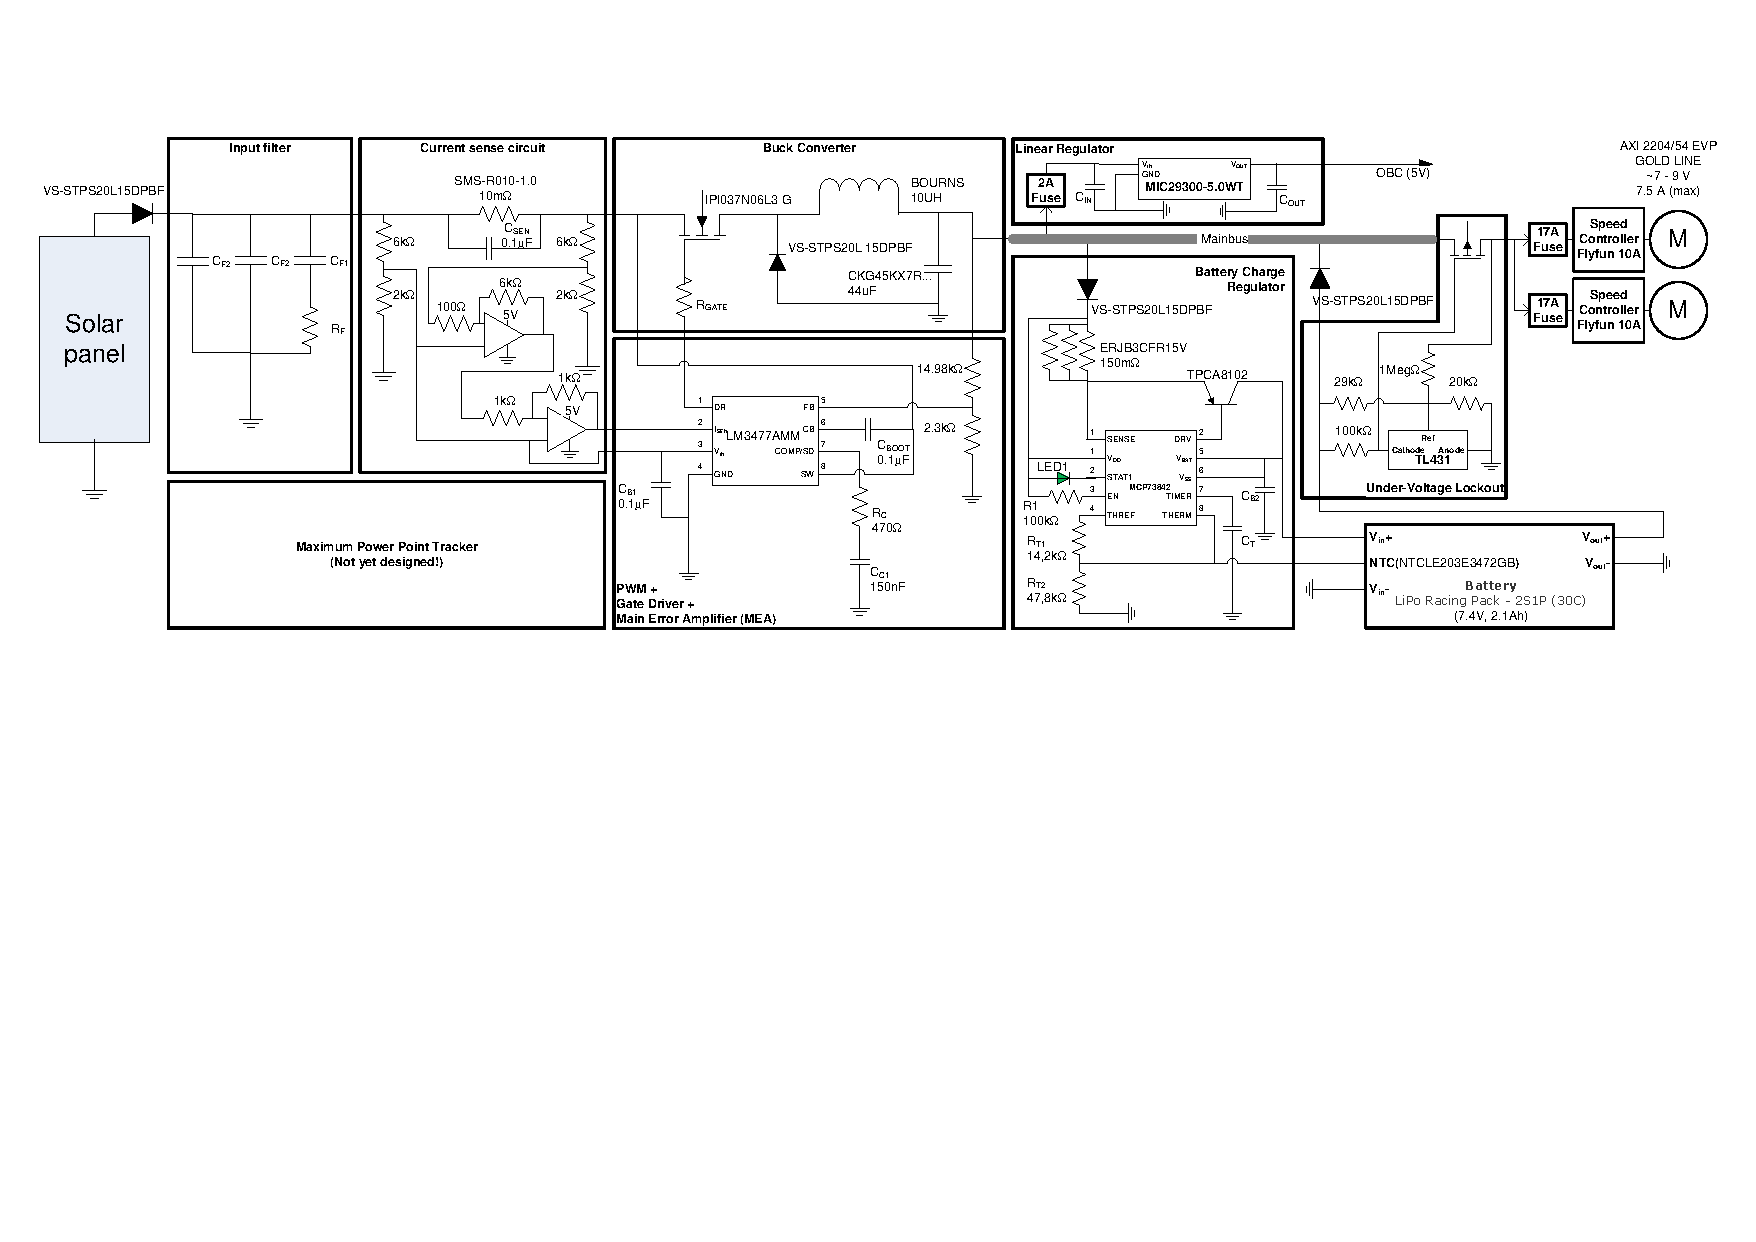
\includegraphics[scale=0.8]{figures/fig_CDR_EPSdiagram_detailed}
\caption{\ac{EPS} detailed block diagram diagram}
\label{fig:EPS_diagram_detailed}
\end{sidewaysfigure}

%
\subsection{External Interfaces}
%
The interfaces of the \ac{EPS} external are listed in table \ref{tab:external_interfaces}.
%
\begin{table}[H]
\centering
\caption{External interfaces}
\label{tab:external_interfaces}
\begin{tabular}{m{0.35\textwidth}m{0.55\textwidth}}
\hline
\textbf{External interface} & \textbf{Implementation}\\
\hline
Solar cells mounting & \ac{PSA}\\[2mm]
DC-DC regulators & Mounted on PCB which sits in system housing. Thermal contact points should be included, to remove internal heat dissipation.\\[2mm]
Battery telemetry & Analog signals to Microcontroller\\[2mm]
Mounting of batteries & \ac{TBD}\\
%Output voltage control(reference voltage setpoint) & Analog signal from Microcontroller\\[2mm]
Supply voltages & $6.0-9.2\,V$ (unregulated) and $5.0\,V$(regulated)\\[2mm]
\hline
\end{tabular}
\end{table}
%
%
\subsection{Telemetry and Telecommands}
%What telemetries/telecommands are required/useful for the subsystem? – What data rates/sizes are required?
%
The required/recommended telemetry and telecommands, \ac{EPS} , are listed in table \ref{tab:Telemetry_Telecommands}.
%
\begin{table}[H]
\centering
\caption{Telemetry and telecommands}
\label{tab:Telemetry_Telecommands}
\begin{tabular}{|l|l|l|}
\hline
\textbf{Telemetry} & \textbf{Data rate/frequency} & \textbf{Data size} \\
\hline
Battery voltage & Every 30 sec & 2 bytes\\
\hline
Battery temperature & Every 5 sec & 2 bytes\\
\hline
%Solar array temperature & Every 30 sec & 1 byte\\
%\hline
%Solar array voltage & Every 1 sec(MPPT performance) & 2 bytes\\
%\hline
%Solar array current & Every 1 sec(MPPT performance) & 2 bytes\\
%\hline
\end{tabular}
\end{table}

\section{Test and Verification of Design}
\label{sec:test_verification}

\subsection{Preliminary Verification of Design}

\textit{Will be included in the final version...}

\subsection{Design Models and Verification Methods}

\subsubsection*{PSpice Simulations}
PSpice transient and average simulation models of the \ac{SAR} will be created. These will help in the design and testing of the regulator performance and system stability during transient loading.

\subsubsection*{Development Model}
A \ac{DM} will be build using self-made "mini-mount" pads and mainly surface-mount components, to minimize parasitic effects. System stability will be tested using a Network Analyzer and MPPT performance will be tested in a \ac{TV} chamber cycling the solar array temperature.

\subsubsection*{Flight Model}
If time allows, a dedicated \ac{FM} will be build, using a custom designed \ac{PCB} schematic layout. An optimized \ac{PCB} layout will minimize the system mass and size while maximizing the efficiency and system robustness.

\section{Resources and Scheduling}
\label{sec:resources_scheduling}

\subsection{Main Tasks}

\textit{Will be included in the final version...}

%The main tasks, to implement the proposed \ac{EPS} design, are listed in table \ref{tab:main_tasks}.
%
%\begin{table}[H]
%\centering
%\caption{Main \ac{EPS} design and implementation tasks}
%\label{tab:main_tasks}
%\begin{minipage}{\textwidth}
%\centering
%\begin{tabular}{|p{0.05\textwidth}|p{0.5\textwidth}|p{0.15\textwidth}|p{0.2\textwidth}|}
%\hline
%\textbf{No.} & \textbf{Task} & \textbf{Duration [days]}\footnote{1 day = 8 effective working hours} & \textbf{Dependence (finish to start)}\\
%\hline
%1 & Design DC-DC regulator & 3 & - \\
%2 & PSpice regulator simulation & 5 & 1 \\
%3 & Order components and produce mini-mount patches\footnote{small pieces of PCB, with sticky bottom, very suitable for high frequency circuit prototyping} & 1 & 1, 2\\
%4 & Assemble solar cells & 3 & 1, 3\\
%5 & Design battery regulation and protection circuits & 3 & 1\\
%6 & Build and test battery circuits & 2 & 3, 5\\
%7 & Build prototype regulator (without MPPT) & 3 & 1, 3\\
%8 & Test prototype regulator (without MPPT) & 3 & 1, 2, 7\\
%9 & Design and build MPPT & 5 & 7\\
%10 & Test MPPT & 2 & 9\\
%11 & Design custom PCB layout & 2 & 1, 5, 9\\
%12 & Manufacture PCB and mount components & 3 & 11\\
%\hline
%\end{tabular}\par
%\vspace{-0.75\skip\footins}
%\renewcommand{\footnoterule}{}
%\end{minipage}
%\end{table}

\subsection{Parts List and Costs}

\textit{Will be included in the final version...}

%The preliminary parts list for the \ac{EPS} is listed in table \ref{tab:parts_list}.

%\begin{table}[H]
%\centering
%\caption{Main \ac{EPS} design and implementation tasks}
%\label{tab:parts_list}
%\begin{minipage}{\textwidth}
%\centering
%\begin{tabular}{|m{0.25\textwidth}|m{0.3\textwidth} |m{0.15\textwidth}|m{0.2\textwidth}|}
%\hline
%\textbf{Part} & \textbf{Part No.} & \textbf{Cost[SEK]}\footnote{cost per piece, hence total cost may be significant higher, depending on required quantity} & \textbf{Reference} \\
%\hline
%Solar cells & MC-SP0.8-NF-GCS & 61 kr & www.farnell.com\\
%Battery & PA-LN19 & 326 kr & www.farnell.com\\
%PWM controller & \ac{TBD} & - & - \\
%Power MOSFET & TBD & - & - \\
%Power diode & TBD & - & - \\
%MOSFET gate driver (high side) & TBD & - & - \\
%OpAmps (feedback regulators) & LT1498 & 92 kr & www.farnell.com \\
%Main bus capacitors & CKG45NX7R1H335M & 38 kr & www.farnell.com \\
%COTS DC-DC converter & IK1205SA & 39 kr & www.farnell.com\\
%Inductor core(s) & TBD & - & -\\
%Current sensor & TBD & - & -\\
%PCB & TBD & - & - \\
%%\hline\hline
%%Total & & ??? & \\
%\hline
%\end{tabular}\par
%\vspace{-0.75\skip\footins}
%\renewcommand{\footnoterule}{}
%\end{minipage}
%\end{table}

\subsection{Electronics Ground Support Equipment (EGSE)}
%
\textit{Will be included in the final version...}
%%
%%
%\begin{itemize}
%\item Laboratory equipment, i.e. Network Analyzer, Digital Oscilloscope, power supplies, multi-meters
%\item \ac{TV} chamber
%\end{itemize}
%%
%\subsection{Mechanical Ground Support Equipment (MGSE)}
%%
%\begin{itemize}
%\item \ac{PCB} manufacturing facilities, i.e. UV light source, etching facility, punch-through hole machine, photo-resist
%\end{itemize}

%\section{Power Distribution Block Diagram and Redundancy}
%
%Block diagram of the different power consumers...
%
%\section{Electrical Circuits}
%
%Explanation of all different circuits involved in the EPS subsystem...